%%    _____  _____
%%   |  __ \|  __ \    AUTHOR: Pedro Rivero
%%   | |__) | |__) |   ---------------------------------
%%   |  ___/|  _  /    DATE: November 10, 2021
%%   | |    | | \ \    ---------------------------------
%%   |_|    |_|  \_\   https://github.com/pedrorrivero
%%

\section{Fermion-qubit mappings}

%% ----------------------------------------------------------------------------
%% ----------------------------------------------------------------------------

\begin{frame}{Fermion-qubit mappings}

	Generally speaking, quantum computers cannot work with any given operator directly. Therefore, in order to simulate this or any other Hamiltonian in a quantum processor, one needs to efficiently map its component operators onto ones suitable for operating in such machines. The most commonly used of these is the \textbf{Pauli set}.

  \begin{center}
    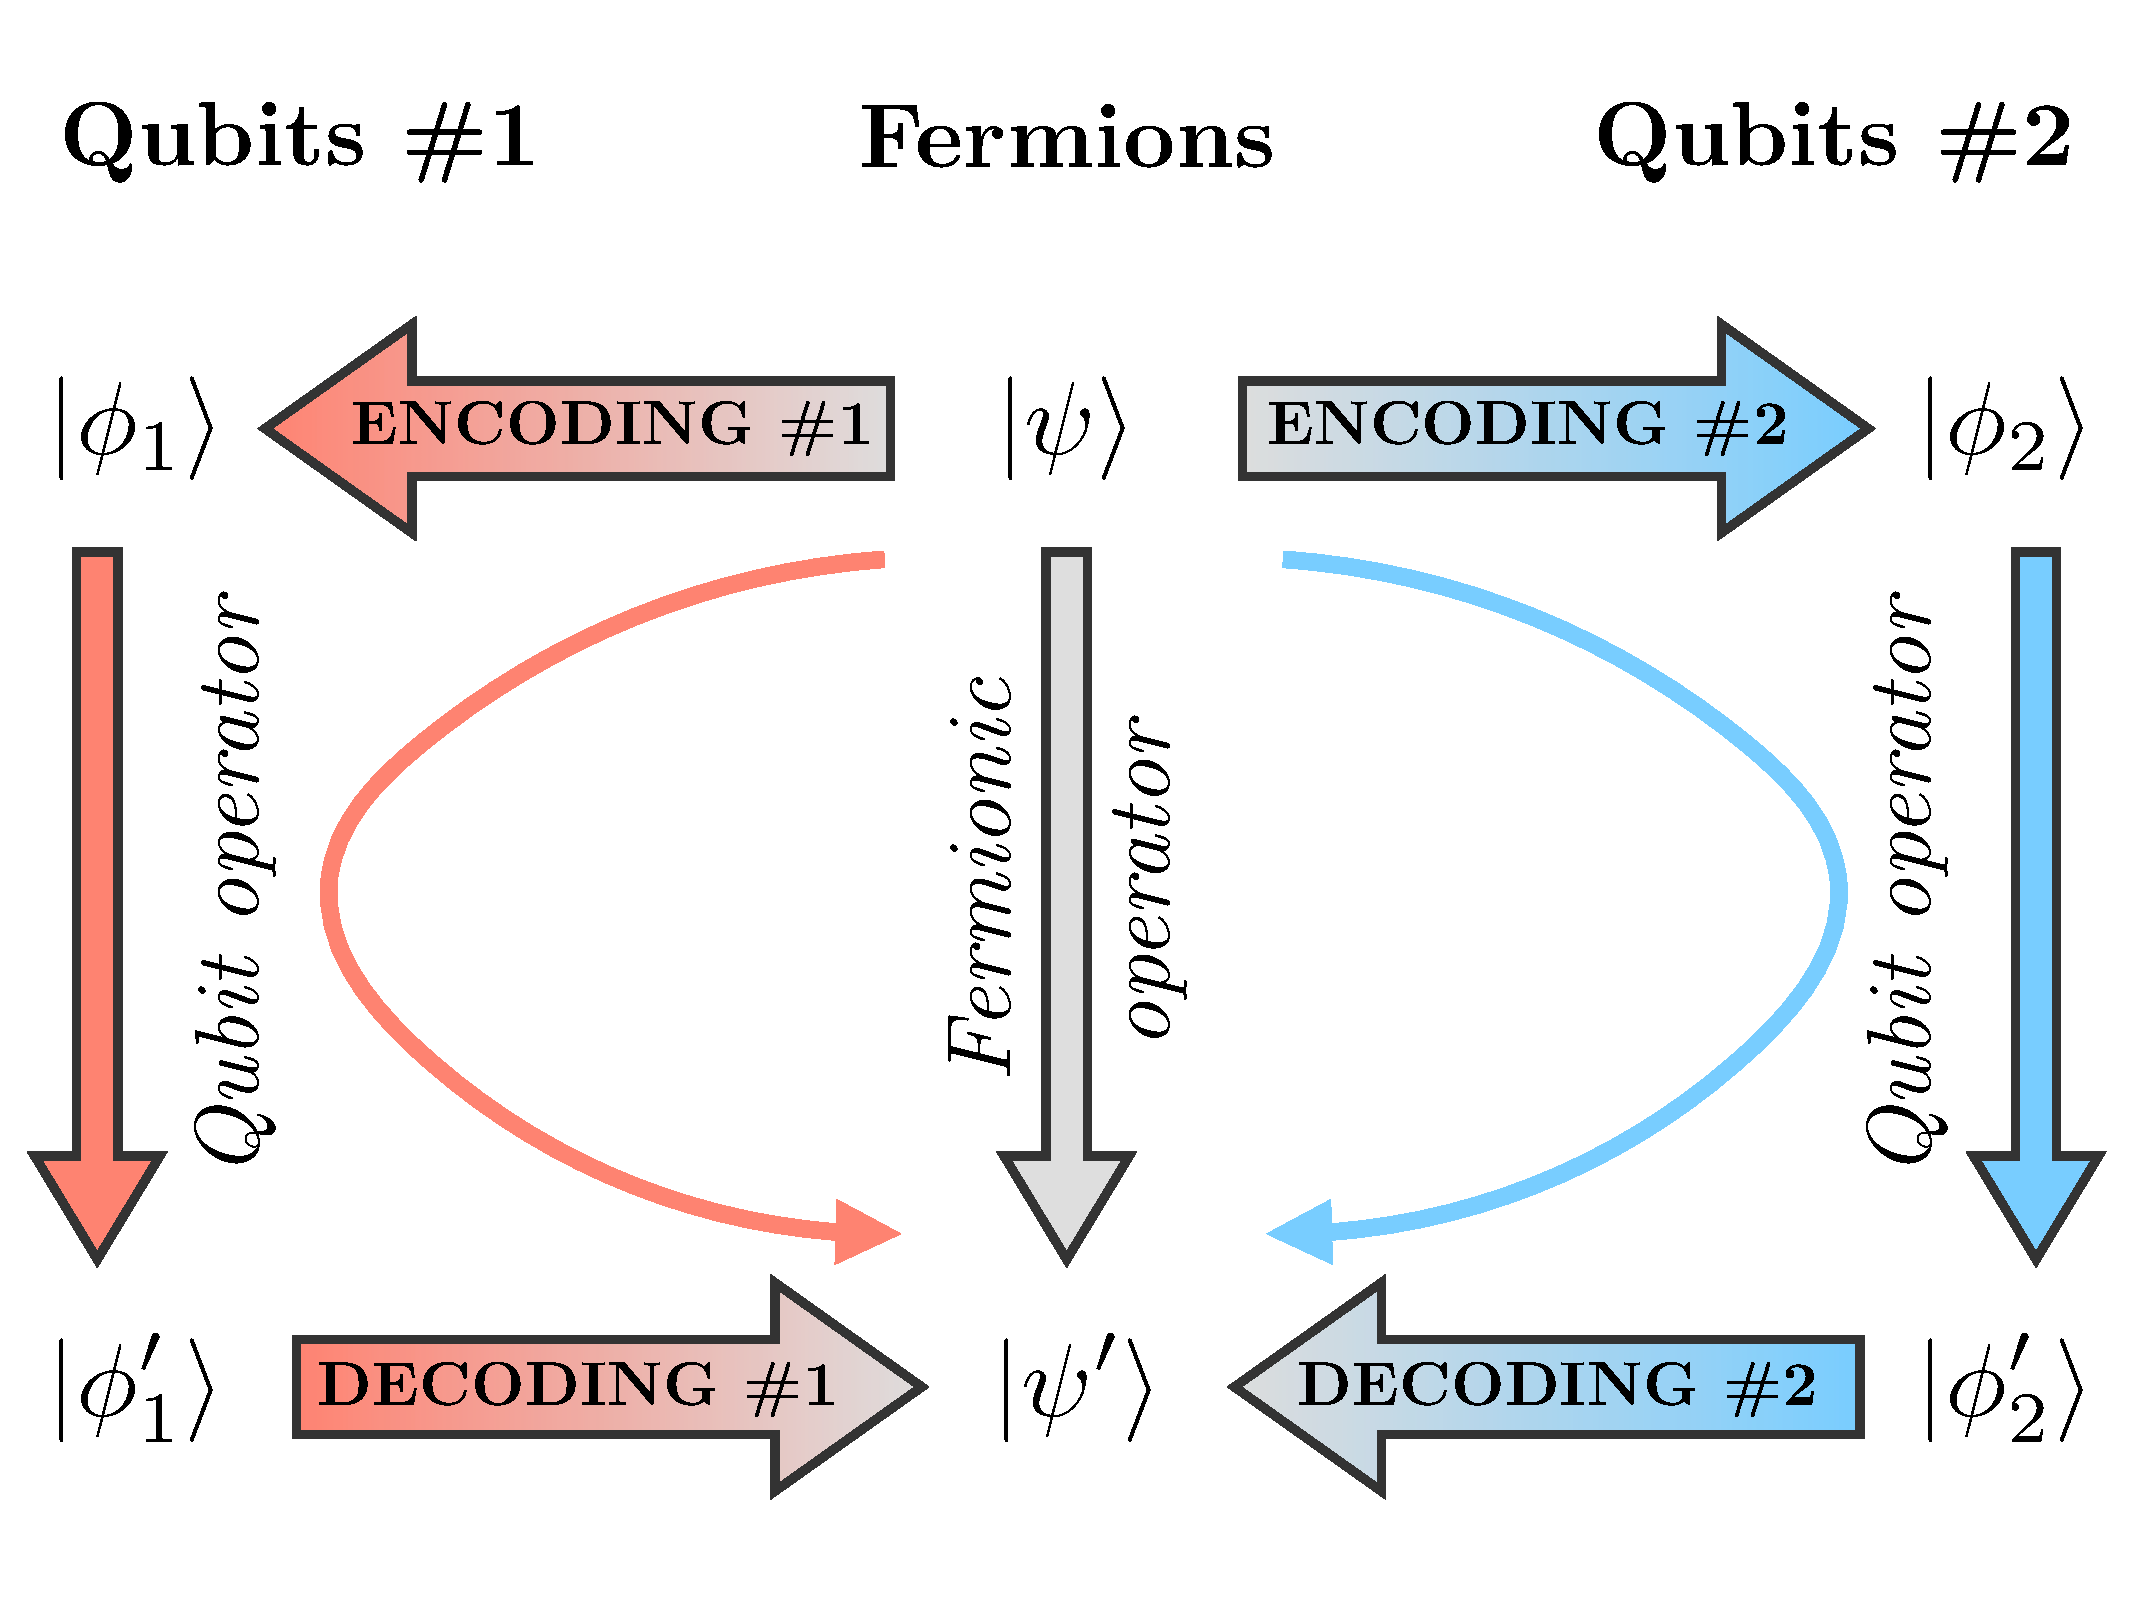
\includegraphics[width=.40\paperwidth]{Figures/chapter03/simulation-mapping}
  \end{center}

\end{frame}


%% ----------------------------------------------------------------------------
%% ----------------------------------------------------------------------------

\subsection{Jordan--Wigner mapping}

%% ----------------------------------------------------------------------------

\begin{frame}[allowframebreaks]{Jordan-Wigner mapping}

  The Pauli exclusion principle introduces a powerful liaison between fermions in the same quantum state. For this reason, even a non-interacting gas of fermions is still highly correlated. However, it turns out that in one spatial dimension spin-$\frac{1}{2}$ particles (i.e. qubits) behave much like fermions. Particularly, we choose:

  \begin{align*}
    \ket{\ua} \equiv \ket{0} &\qc
      \ket{\da} \equiv \ket{1} \\
    \ket{\da} \equiv \phi^{\dagger}\ket{0} &\qc
      \ket{\ua} \equiv \phi\ket{1} \\[5pt]
    \phi \ra \sigma^{+} &\qc \phi^{\dagger} \ra \sigma^{-}
  \end{align*}

  The mapping that the Jordan--Wigner transform introduces is designed on the \textbf{occupation number basis}, which associates spin ``down'' and ``up'' with occupied and unoccupied fermion states respectively. All this allows us to use these spins as a basic model for fermions:

	\begin{gather*}
	  \acom{\phi}{\phi^{\dagger}} = 1 \qra \acom{\sigma^{+}}{\sigma^{-}} = 1
	\end{gather*}

%% ----------------------------------------------------------------------------
\break
%% ----------------------------------------------------------------------------


	% To prove that this is valid, we can define the following equivalences by drawing inspiration from raising and lowering operators in angular momentum theory:
  %
	% \begin{align*}
	% 	\sigma^{1} &\equiv \phi^{\dagger} + \phi \\
	% 	\sigma^{2} &\equiv i\qty(\phi^{\dagger} - \phi) \\
	% 	\sigma^{3} &\equiv 1 - 2\phi^{\dagger}\phi
	% \end{align*}
  %
	% Making use of the properties of fermion creation and annihilation operators, comprised within their canonical commutation relations, these can be shown to behave algebraically like \textbf{Pauli matrices}:
  %
	% \begin{align*}
	%   \com{\sigma^{p}}{\sigma^{q}} &= 2i\epsilon_{pqr}\sigma^{r} \\
	%   \acom{\sigma^{p}}{\sigma^{q}} &= 2\delta_{pq}
	% \end{align*}

%% ----------------------------------------------------------------------------
% \break
%% ----------------------------------------------------------------------------

	% We can recover the usual spin raising and lowering hermitian conjugate operators:
  %
	% \begin{gather*}
	%   \sigma^{\pm} \defeq \frac{1}{2}\qty(\sigma^{1} \pm i\sigma^{2})
	% \end{gather*}
  %
	% All this allows us to use these spins as a basic model for fermions:
  %
	% \begin{gather*}
	%   \acom{\phi}{\phi^{\dagger}} = 1 \qra \acom{\sigma^{+}}{\sigma^{-}} = 1
	% \end{gather*}
  %
  % \break

	Unfortunately, this only works for single-fermion representations; since independent spins commute, while independent fermions anticommute.

	\begin{gather*}
	  \com{\sigma^{+}(p)}{\sigma^{-}(q)} = \delta_{pq} \qc
	    \acom{\sigma^{+}(p)}{\sigma^{-}(q)} \neq \delta_{pq} \\
	  \com{\phi(p)}{\phi^{\dagger}(q)} \neq \delta_{pq} \qc
	    \acom{\phi(p)}{\phi^{\dagger}(q)} = \delta_{pq}
	\end{gather*}

%% ----------------------------------------------------------------------------
% \break
%% ----------------------------------------------------------------------------

	A way to fix this issue is by defining $N(l)=\phi^{\dagger}(l)\phi(l)$ as the hermitian number operator for state $l$, and attaching a so called unitary \textbf{string operator} $S(n)$ to the fermion operators:

	\begin{gather*}
		\begin{split}
			S(n)\phi(n) \ra \sigma^{+}(n) \qc
			\phi^{\dagger}(n)S^{\dagger}(n) \ra \sigma^{-}(n)
		\end{split} \\
		S(n) = \exp[ -i\pi {\textstyle\sum_{l<n}} \qty[N(l)+s(l)] ]
	\end{gather*}

	The $s(l)$ terms in the string operator are scalars associated to \textbf{gauge transformations}.% and do not add much to the transform.% With this new mapping, Pauli matrices get redefined to:

	% \begin{align*}
	% 	\sigma^{1}(n) &\equiv
	% 		\phi^{\dagger}(n)S^{\dagger}(n) + S(n)\phi(n) \\
	% 	\sigma^{2}(n) &\equiv
	% 		i\qty[\phi^{\dagger}(n)S^{\dagger}(n) - S(n)\phi(n)] \\
	% 	\sigma^{3}(n) &\equiv
	% 		1 - 2\phi^{\dagger}(n)\phi(n)
	% \end{align*}

%% ----------------------------------------------------------------------------
\break
%% ----------------------------------------------------------------------------

	We now retrieve the correct statistics. Of course, we would like to express the string operator in terms of the Pauli set so that we can move it to the other side of the transformation. Fortunately, we can do so by expanding the number operators:

	\begin{gather*}
	  \exp[\pm i\pi \sum_{l<n} N(l)] =
		  \prod_{l<n}\exp[\pm i\pi \phi^{\dagger}(l)\phi(l)] =
		  \prod_{l<n}\qty[1-2\phi^{\dagger}(l)\phi(l)] =
		  \prod_{l<n}\sigma^3(l) \\
		S(n) = \prod_{l<n} e^{-i\pi s(l)} \sigma^3(l)
	\end{gather*}

	Finally, our \textbf{choice of gauge} will be such that $s(l) = s \in (-1,1]$ $\forall l$ and the string operator is hermitian for all values of $n$. All in all, this can be achieved by making $s=0$, which gives:

	\begin{gather*}
		\phi(n) \ra \qty[\prod_{l<n} \sigma^3(l)]\sigma^{+}(n) \qc
		\phi^{\dagger}(n) \ra \qty[\prod_{l<n} \sigma^3(l)]\sigma^{-}(n)
	\end{gather*}

%% ----------------------------------------------------------------------------
% \break
%% ----------------------------------------------------------------------------

  % Lastly, we need to bring back flavor indices. The form of the transform will in fact be the same but, for clarity, we would like to write them down them explicitly. This will prove to be useful when dealing with the periodic boundary conditions. For this, all we need recalling is that the flavor sub-lattices had been stitched back-to-back in the final computational lattice:
  %
  % \begin{gather*}
  %   \phi_\alpha(n) \ra S_\alpha(n) \sigma_\alpha^{+}(n) =
  %     \qty[\prod_{\beta=0}^{\alpha-1} \tilde{\sigma}_\beta^{3}(2N)]
  %     \tilde{\sigma}_\alpha^{3}(n) \sigma_\alpha^{+}(n) \\
  %   \phi_\alpha^\dagger(n) \ra S_\alpha^\dagger(n) \sigma_\alpha^{-}(n) =
  %     \qty[\prod_{\beta=0}^{\alpha-1} \tilde{\sigma}_\beta^{3}(2N)]
  %     \tilde{\sigma}_\alpha^{3}(n) \sigma_\alpha^{-}(n)
  % \end{gather*}
  % \begin{gather*}
  %   S_\alpha(n) \defeq S(n + 2N\alpha) \qqc
  %   \tilde{\sigma}_\alpha^{3}(n) \defeq \prod_{l<n} \sigma_\alpha^{3}(l)
  % \end{gather*}

\end{frame}

%% ----------------------------------------------------------------------------
%% ----------------------------------------------------------------------------

\subsection{Refactoring NJL}

%% ----------------------------------------------------------------------------

\begin{frame}[allowframebreaks]{Refactoring the NJL Hamiltonian}

  % Now that we have a way of converting from fermion to spin operators, let's apply it to the NJL Hamiltonian. To do so, we will make use of the Jordan--Wigner transform, and it is convenient to note some previous mappings first:
  %
  % \begin{align*}\begin{split}
  %   \phi_\alpha^{\dagger}(n)\phi_\alpha(n) &\qra
  %     \frac{1}{2} \qty[1 - \sigma_\alpha^{3}(n)] \\
  %   \phi_\alpha^{\dagger}(n)\phi_\alpha(n) -
  %     \phi_\alpha^{\dagger}(n+1)\phi_\alpha(n+1) &\qra
  %     \frac{1}{2}\qty[\sigma_\alpha^{3}(n+1) - \sigma_\alpha^{3}(n)] \\
  %   \phi_\alpha^{\dagger}(n)\phi_\alpha(n+1) &\qra
  %     \sigma_\alpha^{-}(n)\sigma_\alpha^{+}(n+1) \\
  %   \phi_\alpha^{\dagger}(n+1)\phi_\alpha(n) &\qra
  %     \sigma_\alpha^{-}(n+1)\sigma_\alpha^{+}(n) \\
  %   \phi_\alpha^{\dagger}(n)\phi_\alpha(n+1) -
  %     \phi_\alpha^{\dagger}(n+1)\phi_\alpha(n) &\qra
  %     \frac{1}{2i} \qty[
  %       \sigma_\alpha^{1}(n+1) \sigma_\alpha^{2}(n) -
  %       \sigma_\alpha^{2}(n+1) \sigma_\alpha^{1}(n)
  %     ]
  % \end{split}\end{align*}

%% ----------------------------------------------------------------------------
% \break
%% ----------------------------------------------------------------------------

	Hence, bringing back flavor indices, the different parts of the Hamiltonian are:

  \begin{align*}
    H_{N}^{(M)} \qra&
      \frac{m}{2} \sum_\alpha \sum_{n=0}^{2N-1}
      (-1)^{n+1}\sigma_\alpha^{3}(n) \\
    H_{N}^{(K)} \qra&
      \frac{1}{4a} \sum_\alpha \sum_{n=0}^{2N-2}
      \qty[
        \sigma_\alpha^{1}(n+1) \sigma_\alpha^{2}(n) -
        \sigma_\alpha^{2}(n+1) \sigma_\alpha^{1}(n)
      ] + \nonumber\\&
      \frac{1}{4a} \sum_\alpha \!
      \qty[\prod_{l=1}^{2N-2} \!\! \sigma_\alpha^3(l)] \!
      \qty[
        \sigma_\alpha^{1}(0) \sigma_\alpha^{2}(2N \!-\! 1) -
        \sigma_\alpha^{2}(0) \sigma_\alpha^{1}(2N \!-\! 1)
      ] \\
    H_{N}^{(G)} \quad=\quad& - \frac{G_{\pi}}{2a} \sum_{n=0}^{N-1} \qty[
      \sum_{\alpha} \dbtilde{H}_{N}^{\alpha\alpha}(n) + 2
      \sum_{\alpha < \beta} \dbtilde{H}_{N}^{\alpha\beta}(n)] %\\
    % \dbtilde{H}_{N}^{\alpha\beta}(n) \qra&
    %   \frac{1}{4} \sum_{{j=0}\atop{k=0}}^{1}
    %   (-1)^{j+k} \, \sigma_\alpha^{3}(2n+j) \, \sigma_\beta^{3}(2n+k) \qc
  \end{align*}

%% ----------------------------------------------------------------------------
\break
%% ----------------------------------------------------------------------------

  \begin{gather*}
    \dbtilde{H}_{N}^{\alpha\beta}(n) \qra
      \frac{1}{4} \sum_{{j=0}\atop{k=0}}^{1}
      (-1)^{j+k} \, \sigma_\alpha^{3}(2n+j) \, \sigma_\beta^{3}(2n+k) \qc
  \end{gather*}

  It is important to notice that the periodic boundary conditions only enter through the kinetic term, and are responsible for the only non-local contribution. Finally, it is useful to note that:

  \begin{gather*}
    \dbtilde{H}_{N}^{\alpha\alpha}(n) \qra
      \frac{1}{2} \qty[1 - \sigma_\alpha^{3}(2n+1) \, \sigma_\alpha^{3}(2n)] \qc
  \end{gather*}

  which shows an extensive \textbf{adiabatic modification} term of the form $\frac{G_\pi}{4} N_\text{flavor} \times \frac{N}{a}$ in the interaction Hamiltonian (i.e. coming from the unit matrix). This term gathers the two usual singularities from Quantum Field Theory: one with the size of the system as it gets larger (i.e. $\sim N$), and the other on the continuum limit (i.e. $\sim 1/a$). We drop it as a vacuum contribution.

\end{frame}
